%=========================================================================
% (c) Michal Bidlo, Bohuslav Křena, 2008

%\cite{Rybicka}
\chapter{Introduction}
	\section{Overview}
	%descripcion general del proyecto, que busca, como, para qué.
	This project consists on creating an intelligent device able to measure the temperature from a Raspberry Pi board and a temperature sensor. Moreover, the device has to be prepared to create a web server which provides a web platform which shows visitors the last temperature samples taken by the device and also allows logged users to change the configuration parameters of the device remotely.

	The objective of this project is to use a Raspberry Pi board and some hardware components like a RTC module and a Temperature sensor create a device which will be able to get temperature samples of the surrounding place.

	This temperature station has to be prepared to send the data to another target machine and be configured remotely from a web application which has to be provided for a web server hosted also in the same device.

	That Web application will be composed by public area which will show the temperature samples and a graphic to the visitant users and also a private area protected with login which will allow authenticated users to change the device configuration like samples frequency, number of samples shown in the web page or also the target machine for the scp data transfers.

	This project is framed in the field of Internet of the things and thought as a investigation about the capabilities of the well known Raspberry Pi board for host a complex embedded system in an efficient way as a data producer for other devices. The processing of that temperature data is not an objective of the designed system, leaving aside the web page provided by the system which will create a simple graphic with it.

	The system will be designed as a standalone system which will provide all the mentioned features. The system is also thought for being moved to some different locations, reason why the device will be wireless, using a usb Wi-Fi module in order to get connected to Internet and a battery to get the power.

	Furthermore, the power efficiency is another important matter in the project as a consequence of using a battery as a power source, so the system will allow the user to decrease the power consumption changing some device configurations and disabling device functionalities.

	\section{Internet of the Things}

	The Internet of Things (IoT) is a relatively recent concept which refers to the interconnection of devices in the physical world like thermometers, washing machines or traffic lights. This network of devices permits us to create new machines which will do more complex things than we thought possible years ago.

	They IoT network can gather and create a lot of data using the devices sensors in the network which is exchanged between devices. Also, these devices use other devices data to choose the best behaviour in every case permitting the machines to becoming more intelligent which means that it can automatice more tasks, give us more and more useful information and becoming more accurate and efficient making their tasks.

	One of the facts that are responsible for the success of the IoT movement is the hardware requirement. The IoT promotes the use of little embedded hardware devices which limit CPU computational power, few memory and also low power consumption. This is a real advantage comparing to other kind of systems which require expensive and powerful machines and permit to integrate IoT systems in almost all the fields. Some of the most useful fields are in industry automating task, in the domestic field for example helping to consume energy in an efficient way or notifying a broken electrodomestic. Also it can be used to get environmental information which can help to get advised of a natural disaster before it happens or to control the water contamination. One more important field is set in urbanism, this technology permits us to get many useful information, for example, about traffic, contamination and pollen in the air. This examples are only a few comparing to the real possibilities of this technology. 

	Other of the important facts which permitted to start thinking of IoT as a serious alternative was the release of IPv6 addresses allowing this little devices to get access to Internet and permitting to interconnect these devices between them no matter the distance and location. And more important, permitting users to manage and get information of these devices from every place. This last advantage also carries an important matter concerning to the security of the information which is generated by this devices and also for protect this devices against malicious persons who can get advantage of use them for their own interest.

	Between the reason which are making this technology grow, one is the scalability of these networks. It is relatively easy to add new devices to the network which will generate more data or use the existent data for increase the functionality of all the network. %TODO de ser necesario aqui se tiran dos parrafos mas.

	Nowadays, many companies are becoming to release new IoT products which greatly improves the life of the users.
	There are many examples like intelligent fridges which notify the owner when there isn't any bottle of milk. Or the example of sensors which measure the toxicity of the river wate preventing us to get poisoned from a factory leak. And also systems which using a smartphone application allows a driver to know where is a place to park the car.

	One particular example of these technologies can be found in Santander, Spain, where the parkings are intelligent. There are sensors under the floor which send the status information of the parking to a server which makes this information public to the inhabitants.

	Also in Zaragoza, Spain, sensors gather anonymous information about the places where people usually go, from where and at what time in order to improve the public transport.

	This last example also carries some considerations about the privacy of the people when these systems are introduced in our lives, how this data can be used and which limits we have to put. %TODO aqui tambien puede meterse otro par de parrafos.

	\section{The aim of this project}
	There are many alternatives to make an embedded system, from specific chips which perform particular and fixed tasks, or more general chips like Arduino which allows to perform more complex tasks and manage other sensors and finally devices like Raspberry Pi which are computers with full functionality and capabilities with low power consumption and a litle size.

	This project has been planified in order to test devices like Raspberry Pi, which are becoming more powerful and efficient day by day allowing to create new and more complex devices with more possibilities than traditional embedded systems.

	The problematic of the topic is the management to make a power efficient system. A simple embedded system will consume much less power than a device like Raspberry Pi which is composed by many chips. But the possibilities of a system deployed in a Raspberry Pi are incredibly bigger than one ``system'' deployed in an embedded chip or an Arduino board due to the greater capabilities of Raspberry Pi board that can be so useful in the IoT field which is growing fastly and demanding more complex functionalities every day.

	It is important be concerned about the security and safety of the data stored in the device. Credentials, certificates and also the samples. In the moment our system is designed to be located in every place wirelessly it is important to start thinking about not only to protect this data from online hacker but also to protect it against people who manage to steal the physical device and access to the data physically.

\chapter{The system: Hardware}
	\section{The Raspberry Pi} %TODO fix entradilla
	Raspberry Pi is a well known micro computer which has become famous due to its low price and its high performance in a device of this size and price characteristics. After years of its releases the community behind it continues growing and growing and because of that fact combined to the possibilities that this device characteristic offer has created a great context to develop small smart devices at a low price, fact which becomes Raspberry Pi in a great choice for IoT projects.

		\subsection{History \& social importance}
		The creator of this device was Eben Upton realized that new students of computer sciences in Cambridge University had lower computer skills. Upton arguments that this is because the new game consoles, mobile phones are ``fixed function devices'', not like the old devices such as Commodore or Spectrum which users needed to learn how to programm it in order to use it.

		To solve this problem he proposed a new little machine that could be bought for a low price, like 25\$, which could help child to learn about computation and programming. The success of this idea was completely unexpected for Embed Upton who thought about creating only 1000 devices. In the first day after the release, they sold 100.000 devices.

		Nowadays, the Raspberry Foundation is supported by the University of Cambridge Computer Laboratory and Broadcom, which is an educational charity meant to promote the study of computer science topics using Raspberry Pi as a tool.

		Right now, many organizations use Raspberry Pi with an education purpose in all education levels and every time more countries are using it in the schools as a tool to teach children not only computational skills but also mathematical concepts and other fields like physics with tools such as the Scratch programming language.

		This cheap device has created a huge community of people around it who are interested in using it as an education tool, as a research device and also as an entertainment tool. And actually it is possible to learn how to build interesting and complex projects thanks to it. There are many examples and ideas which also started as a kind of entertainment and ended up as a commercial product.

		\subsection{Hardware}
		The Raspberry Pi is a fully functional computer with also a low power consumption. Since the first one was released, several new models have appeared. The first one was the model A, then the model B, A+, B+, model 2 B, 2 B + and recently models Zero and 3.
		Every model has a different hardware design. There had been some improvements among them. The model used in this project is the Raspberry Pi 2 B+, which is not the choice that fits better in this project as I explain in the \ref{subsec:powersave} subsection.

		In this section i will explain briefly the main hardware characteristics of the model used in the project.

		\begin{figure}[h!]
		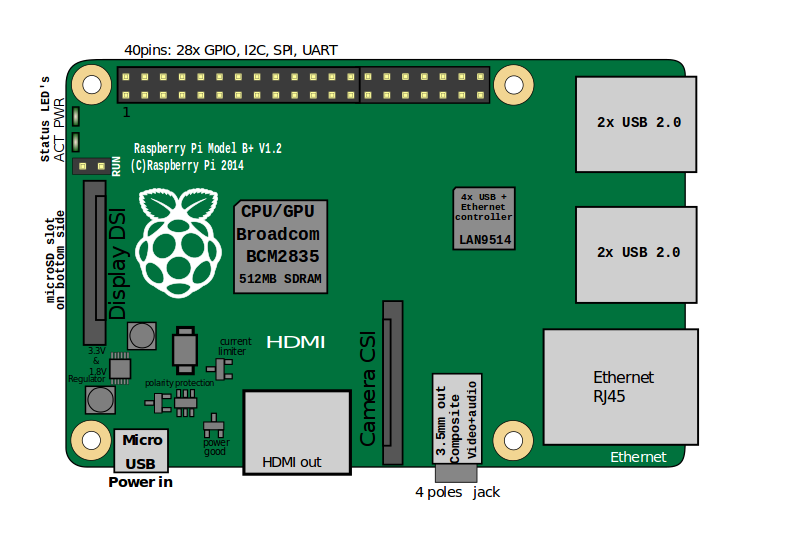
\includegraphics[width=8cm]{fig/rpi2hw.png}
		\centering
		\caption{Raspberry Pi main components.\label{fig:rpi2hw}}
		\end{figure}

		The board, by default, builds four USB ports which allow it to handle multiple peripheral connections like keyboard, mouse, Wi-Fi usb module and others. There is also a micro USB port but is designed to power the device with a standard smartphone charger.

		In order to allow the Internet connection the device mount an ethernet socket. In our project it was needed to buy also a USB Wi-Fi module to allow the device to be moved everywhere without depend of any unnecessary wire.

		Both, the USB ports and the ethernet socket, are controlled by the same hardware hub. This fact was important in the develop of the power saving modes as it is explained in section \ref{subsec:powersave}.

		There are also other connections which are not used in this project like the 3.5mm audio jack and composite video port, the Camera interface (CSI) and the Display interface (DSI). Also there is a HDMI port which was used for the development and it will probably use for the maintenance in the future but it is not used while the device is running normally.

		The principal data storage of the device is in a microSD card, the board also counts with a micro SD card slot.

		The CPU mounted in the Raspberry Pi 2 B is a ARMv7 quad core at 900 MHz and the principal memory is a 1 GB SDRAM at 400 MHz.

		Finally, the board has 40 GPIO pins, these pins are one of the most important features in the machine, which permit to add a new hardware, sensors and controllers to the board allowing to develop complex systems as robots, media centers or weather stations.

		\subsection{Power save works}\label{subsec:powersave}
		As a micro computer the Raspberry Pi board has a low consume of power. Because of that, this device is a great option for build systems which has to work full time without stop. But in our system, the power is one of the strongest limitations since the device will use an external battery as power supply. 
		
		For our project, the device has some hardware components which we do not need, like the HDMI socket or all the USB ports less one for the Wi-Fi usb module. After the research, it is possible to disable these components saving some battery and some of the power modes disable it as we have explained in the \ref{sec:powersavingmodes} section. 

		Although there is a limitation, USB ports are not independent between them and with the ethernet socket. This is because all of these ports are controlled by the same hub. So when we disable the power we can not disable only one of them and we will lose any possibility of having Internet connection because our two ways to get this are the ethernet socket and a USB Wi-Fi module which uses one of these four USB ports.

		This dessign was made thinking in the mobile systems and it is simpler than a normal desktop computer USB hub and it does not allow to only let one of the usb ports enabled. It is possible to disable the data transmission of the ports but the device will continue giving them energy so it is not useful to disable them. How i will explain in possible improvements disable the data transfer would be useful as a security functionality. %TODO linkear a possible improvements que sera en conclusions vamos.

		On the other hand so many Internet blogs write about downclock the CPU frequency, in the practice downclock the Raspberry Pi CPU saves a despicable amount of power but the heat of the CPU decreases and this fact can avoid corrupt the temperature samples.

		\begin{figure}[h!]
		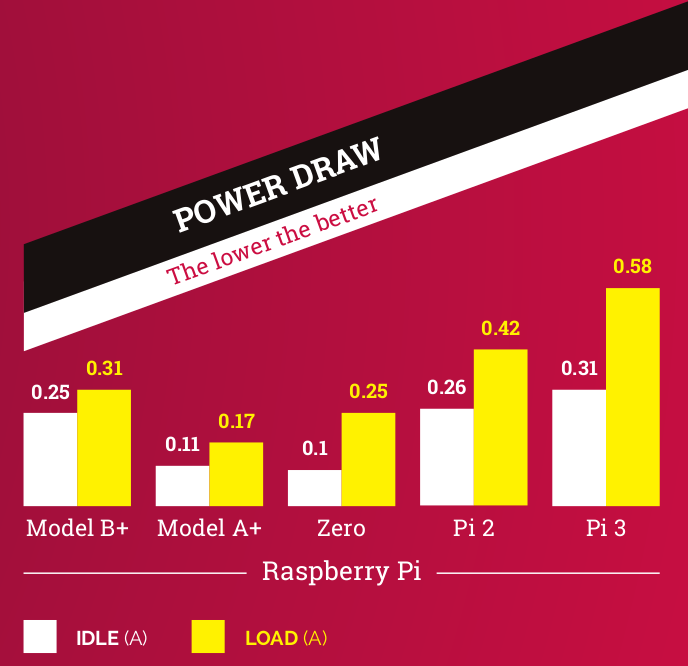
\includegraphics[width=8cm]{fig/powerdraw.png}
		\centering
		\caption{Power consumption diagram from Raspberry Pi Magazine.\label{fig:powerdraw}}
		\end{figure} %TODO link caption to bib

		Other save method is to disable the status led which decrease a bit more the power consumption but at the end is also a despicable amount.

		As a final consideration, there is a Raspberry Pi model, the model A, which is more suitable for this project. That model has a lower regular power consumption than the B model and only had one USB between other facts as show in the \ref{fig:powerdraw} figure.


	\section{The Module}
		\subsection{Installation}
		The provided module comes prepared to directly plug in the Raspberry Pi GPIO pins. The module has to be plugged in the 1, 3, 5, 7 and 9 pins according to the module installation manual. 

		This will allow us to access and install the two components pf the module. The first one is a RTC module model PCF85163 which can be configured to keep the right time between reboots and also to release alarm signals in the right moment. The second chip in the module is a temperature sensor model DS18B20 which is a one-wire digital sensor that measure the temperature.
		
		\subsection{PCF85163}
		The PCF85163 is a CMOS Real-Time Clock (RTC) and a calendar optimized for low power consumption. Although, this chip provides other functionalities, the two functions which the system use of pcf85163 are the clock output which permit to get the actual date in the pcf85163 and the interrupt output which permits to wake up the device from a sleep state.

			\subsubsection{Why a RTC?}
			Our system needs to still work after several days but the Raspberry Pi device despite being a device which consumes so few battery comparing to a normal computer, consumes so much battery comparing to a hardware specialized for embedded systems. For this reason we need to low the consume of the device in order to save battery to maintain working out the device more time. 

			Carrying this to an extreme, one of our partial objectives is to make the device consume just the necessary battery to make its job.

			In order to achieve this partial objective, the way to consume the less battery as possible is putting the device to sleep in the intervals when the user does not need to interact with the device and it is supposed not to run a task.

			Normal computers have a special hardware which permits them to wake up automatically when they are sleeping. Unfortunately, the Raspberry Pi does not count with the necessary hardware for wake up automatically. That is the reason why we need a RTC, which allows the Raspberry Pi device to wake up using his interrupt output which sends a signal to device when a configured alarm occurs.

			\subsubsection{PCF85163 Chip} %TODO FIXME

			How is represented in the figure \ref{fig:pcf8563-pins}. The chip count with 8 pins.

			\begin{figure}[h!]
			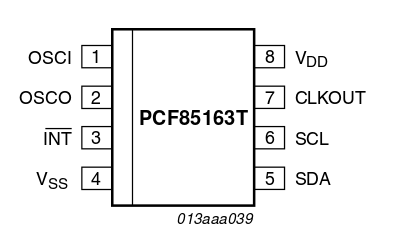
\includegraphics[width=8cm]{fig/pcf85163t.png}
			\centering
			\caption{PCF8563 pins diagram.\label{fig:pcf8563-pins}}
			\end{figure}

			The fourth and the eight pin are from the ground and the power. The first and the second pin are the input and output of the chip oscillator. The seventh pin is the clock output and the fifth and sixth are the serial data I/O and the serial clock input. The third pin is the alarm output which only will be activated when the alarm happeds.

			\subsubsection{Installation}
			The pcf85163 comes also build on a prepared module for Raspberry Pi. For this reason once the module is plug on the Raspberry Pi is necessary to add \texttt{dtoverlay=i2c-rtc,pcf8563} in the \texttt{/etc/config.txt} file.

			This line in the device configuration will mount the modules for manage RTC modules in the system and the specific drivers for control RTC chips of the pcf8563 family.

			Then, after reboot the device, is necessary to configure the actual time stored in the chip, for this task we can synchronize with the system time if it is updated or set up the time manually. Some Linux distributions as Raspbian offer an interface for this using with the command \texttt{hwclock}. For set the system time in the chip we can use \texttt{hwclock -w} command. For set it up manually we can use \texttt{hwclock --time --set="date"}.

			After setting up the correct time, we have to configure the device to get the time of the RTC module on boot time. To get this we need edit \texttt{/lib/udev/hwclock-set} and change all the \texttt{``--systz''} apparitions for \texttt{``--hctosys''}.

			Now it is possible to access to the RTC time and apparently the time is keep between reboots but it is not the reality. In this kind of device like raspberry pi, which does not have any hardware clock for keep the actual time, exist a process called \texttt{fake-hwclock} which calculate the actual time.
	%TODO mirar esto de abajo y ponerlo como bloque de codigo y no asi todo feo
			For force the system to use the RTC module time we have to remove the \texttt{fake-hwclock} process from the system using the following commands.\\\\
			\texttt{sudo apt-get remove fake-hwclock}\\
			\texttt{sudo rm /etc/cron.hourly/fake-hwclock}\\
			\texttt{sudo update-rc.d -f fake-hwclock remove}\\
			\texttt{sudo rm /etc/init.d/fake-hwclock}\\
			\texttt{sudo update-rc.d hwclock.sh enable}\\\\

			Now the system will get the time from the RTC however the time of the system in every reboot is always ``Jan 1st 1970''. This happen because before set the hour from the RTC in the system, the RTC time is overwritten in \texttt{/lib/udev/hwclock-set}. For fix this it is necessary to remove or comment the following lines in the script.\\\\
	%TODO fix this
			\texttt{if [ -e /run/systemd/system ] \; then}\\
			\texttt{exit 0}\\
			\texttt{fi}\\\\

			Now the RTC keep the right date and the system gets the time from the RTC properly.

			\subsubsection{How use it} %TODO validar el comando para obetener el tiempo del rtc
			There are multiple ways for use it, in our project get the date from the RTC is made automatically from the system once it is configured so we do not need to manage with this. Although the time can be get using the command \texttt{hwclock -r} or getting the value of the file \texttt{/sys/class/rtc/rtc0/time}

			Also we need to configure the alarms in the RTC in order to wake up the Raspberry pi in the right moments. This last task is not trivial and needs low level programming so that the development os this was considered as out of the scope of the project. For achive this i used a library called ``AlarmPi'' which provide the necessary interface for manage alarms in the RTC module. This library uses Python3 instead of Python 2.7, this is not a real problem because Raspbian and most of the Debian flavours bring by default both.

			``AlarmPi'' has a useful script called \texttt{setAlarm.py} which permit to set the alarm in the chip for a specified day in the month, recover the scheduled alarm time from the chip and also erase the alarm from the device. The command for set the alarm which is the command we need is \texttt{python3 setAlarm.py -d day -h hour -m minute} allowing us to set an alarm in a specific day of the actual month and for a specified hour and minute. The hour must be set up in a 24 hours format. Finally for cancel the actual alarm is necessary to use the ``-c'' flag (``--cancel'') without any value and for recover the alarm from the chip the ``-s'' flag (``--status'').

			\subsubsection{Problems during the development} %TODO revision de samuel. poner  + paja para disimular?
			The RTC installation consumed so much time, the instructions sum up here are the product of a hard investigation. The main problem was the lack of information about this module not only in Internet blogs because it is not a well known module, also in the store web page there is not referent to the fabricant and the documentation provided does not provide enough information for a developer.

			Also the first module provided has a manufacturing defect which allow to get the temperature value of the sensor but does not permit to get the values from the pcf85163 RTC returning by the standard output of the \texttt{hwclock} command this following non explicit error.\\\\

			\texttt{hwclock: The Hardware Clock registers contain values that are either invalid (e.g. 50th day of month) or beyond the range we can handle (e.g. Year 2095).}\\\\

			After search the causes and also solutions to this error, try in some other distributions without any modification and try alternative installation methods it was impossible to determine why the RTC fails. Then i tried a copy of the module which worked properly so assumed that was a hardware error.

			Also this module was not designed for wake up the raspberry pi and the board of the module does not connect the pcf85163 alarm output pin to the module output so i managed to connect it wiring the alarm output pin to the ``run'' input of the Raspberry Pi board with the hope of emulate this function. As for today i could not manage to achieve this so the third power saving mode, described in the section \ref{sec:pm3}, will remain as a demo feature, the code of the power mode will be provided as normal but in the script the called mode will be the second one.

			Actually, it is possible to set up and recover the alarms from the chip using the ``AlarmPi'' library but it is not certain whether the RTC is capable of waking up the device using the alarm signal when it happens. The only source of information concerning this topic was the company which created the ``AlarmPi'' library for their own products.

			There are also other modules more complex than the provided one which are specifically created to manage and optimize the power consumption in Raspberry Pi and also to enable hibernation and suspend modes in the device like Sleepy Pi shield board.
			%TODO linkear sleepypi to bib y poner otro ejemplo
		\subsection{DS18B20}\label{sec:ds18b20}

		The main sensor in the system is the DS18B20 temperature sensor. This is a 1-wire sensor and permits to connect various DS18B20 sensors in parallel using the same pins, one for the data and another one for the power. This sensor measures the temperature directly in a digital format permitting to get the data directly from the sensor. This sensor can work in a range of temperature between -10ºC and 60ºC according to the module specifications.

		\begin{figure}[h!]
		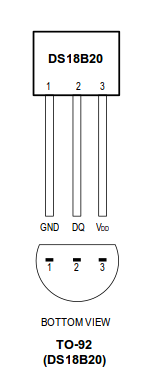
\includegraphics[width=2cm]{fig/ds18b20.png}
		\centering
		\caption{Sensor diagram.\label{fig:ds18b20}}
		\end{figure}

		Moreover, this sensor uses a parasite power mode, which permits it to drain energy from the data bus.

			\subsubsection{Installation}
			First, we need to connect the sensor to the Raspberry Pi. The DS18B20 has three pins as shown in the figure \ref{fig:ds18b20}. The first and third ones are for the 3v3 pin and for the ground pin, the second one, connected to the 4 GPIO transfers the data. The following figure show the connection diagram necessary for this sensor.

			\begin{figure}[h!]
			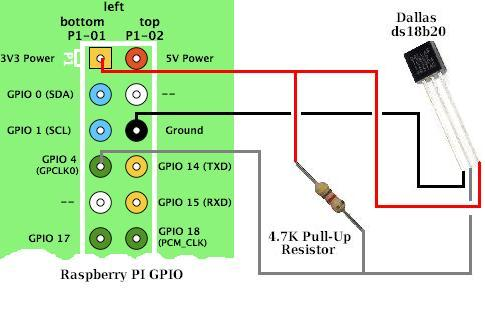
\includegraphics[width=8cm]{fig/ds18b20-connections.jpg}
			\centering
			\caption{Connection diagram for ds18b20 sensor.\label{fig:ds18b20-connection}}
			\end{figure}

			The ds18b20 needs to be wired also with a 4.7K resistor as is written in the documentation of the sensor.
			In our case the sensor was built and ready to use on a RTC module so it was not needed to modify the hardware provided wiring a resistor.

			Once the sensor is physically installed it is necessary to change some configuration files in the Raspberry Pi with the purpose of allow the device to detect the sensor and read from it.

			In order to make this possible we need to add \texttt{dtoverlay=w1-gpio} in the \texttt{/etc/config.txt} configuration file.

			\subsubsection{How to use it}
			Once the sensor is connected and detected by the device, there should be a file in the \texttt{/sys/bus/w1/devices/} folder called \texttt{28-*} being the star a string identificator of the sensor which permits to distinguish between this sensor and another ds18b20 temperature sensors. Inside the sensor folder, if we make a \texttt{cat} of the \texttt{w1\_slave} we will get dump of the sensor data as it is shown in the figure \ref{fig:ds18b20-dump}.

			\begin{figure}[h!]
			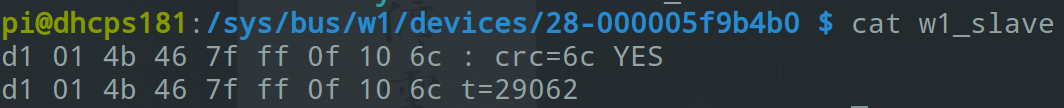
\includegraphics[width=12cm]{fig/ds18b20-dump.png}
			\centering
			\caption{Dump of the ds18b20 sensor data.\label{fig:ds18b20-dump}}
			\end{figure}

			As we can see in the figure \ref{fig:ds18b20-dump} our temperature sensor is the 28-000005f9b4b0 being the identificator of our sensor the \texttt{000005f9b4b0} one. Also in that figure we can see there is written a ``YES'' which means that the data of the sample is not corrupted. Also we can see ``t=29062'' which represents the value of the temperature. To get the right value we have to divide that value between 1000 getting a value of 29.062 ºC.

\chapter{Software decisions}
	\section{The Operative System}
	There are so many options available in the market. Everyone has his own pros and cons but at the end I decided to bet for compatibility and i chos the official Debian flavour designed specially for the Raspberry Pi.
		\subsection{Why raspbian lite?}
		There are so many reasons to choose Raspbian. But the most important is because is a distribution made by Raspberry.org, specially designed for the Rasperry Pi. It means that all the community behind Raspberry Pi is more likely to use this distribution. That is so useful in order to find solutions, tutorials, documentation and libraries specially made to be used in this distribution with a Raspberry Pi device.
		Also it is so useful because the Raspbian distributions count with the called Lite version. This version is offered without graphical interface support, so thanks to this, it does not have to store several unnecessary and expensive drivers in memory and also the image in memory is lighter than the normal one.
		\subsection{Consequences during the develop}
		Working without graphical interface is less comfortable than working with it but after getting used to work only with the shell, the develop were faster. Choosing Raspbian Lite was a really great decision because all the official documentation concerning Raspberry Pi is thought to use this software distribution and even more important it contains all the necessary drivers to work with the Raspberry Pi hardware.

			\subsubsection{Wi-Fi setup}
			VUT University provides two Wi-Fi networks, one is VUTBRNO network and the other one is Eduroam. I prefered use Eduroam because it has Wi-Fi spots in several universities and organisations attached to the project Iris around all Europe and VUTBRNO authentication uses a web formulary which is difficult to fill from the command line or a script.

			The Wi-Fi setup from command line is not as easy as one made from a graphical user interface. After searching the commands or configurations needed to configure the Wi-Fi connection in a distribution without graphical interface as Raspbian Lite i found the wpa\_supplicant command line utility which permits to configure a connection and is used in every reboot for the system so is was perfect to connect the device to Eduroam.

			The setup of the wpa\_supplicant configuration is not so difficult. It is needed a configuration file with the network credentials and security configurations and a couple of commands. The configuration file for the wpa\_supplicant is available in the anexus. %TODO link to anexus and also create the anexus.

			Once the configuration file \texttt{wpa\_supplicant.conf} is created and placed in \texttt{/etc/wpa\_supplicant/} it is only necessary to execute the following commands:\\\\
			\texttt{sudo wpa\_supplicant -Dwext -iwlan0 -c /etc/wpa\_supplicant.conf}\\
			\texttt{sudo dhcpcd wlan0}\\\\

			\subsubsection{Components disable}
			One of the important points in the project is the possibility of move the device everywhere only with a battery suppliying power. This means that we have a important necessity of save all the power possible and develop an efficient system. One of the most important actions was disable all the hardware components that are not needed in the device. Using this distributions disable all the components that the hardware design permits were trivial only using some scripts provided by the distribution.

		\subsection{Other alternatives}
		Raspberry Pi can run several operating systems so that offer huge possibilities. The most well known possibilities are Raspbian, Ubuntu Mate, Windows 10 IoT core and Openelec offered in the official Raspberry Pi foundation web page. Also there is some general alternatives not specifically offered for Raspberry Pi like Debian, Linux Mint, Slackware and Archlinux. 

		After read about the options I prefered to take out Windows 10 IoT because i am not familiarized with the windows environment, Openelect since is specialized in multimedia and the general distributions since they do not offer anything special, have so many things that i do not need and also could need special drivers for interact with the Raspberry Pi.

		Between the specialized options, even if each one offer its own special capabilities, I prefered to use the official distribution for the Raspberry Pi in order to avoid hardware incompatibilities and lacks of documentation.
	\section{The language}
	One of the most important decisions was about what language is most desirable and fits better this project to finish successfully. There was an important matter to choose one language which permit a fast development and works efficiently in the Raspberry Pi.
		\subsection{Why Python?} %TODO improve
		Finally one of the best alternatives was Python. The main reason is that it is already included in the operating system choosed, Raspbian. Thanks to this we avoid occupy more space in memory with another language libraries. 
		Furthermore Python provides a great support and a great amount of libraries to interact with the operating system and the Raspberry Pi hardware. 
		For this reasons Python grants a fast development.
		\subsection{Consecuences during the develop}
		Because my inexperience using Python it was difficult to get use with the use of Python. Despite of that Python solved so many problems simple and efficiently using the default python libraries like the cron library, the daemon library and the cryptographic library.
		\subsection{Other alternatives}
		Other great alternatives were C and JavaScript. The first one provides a low level and so efficient approximation to the problem and it is also by default in the operating system, despite of this the develop using C requires more time and i am not familiarizated with it. In the other side JavaScript would be a great option using also NodeJS. Also JavaScript provides great libraries and it is so comfortable for the developer to develop backend and frontend in the same language but it is not focus in interact with the operating system, there is not information about performance and power consumption in Raspberry Pi and it is not included in the operating system by default.
	\section{The web server}
		This decision was conditioned by the code language chosen. The problem was to decide between all the possibilities based in python assuming also that we need a so efficient and lightweight server.
		The web server have to provide static web pages and the web application needs to have a public part with the data and some graphics and also a private part where it is possible to change the device configuration like power saving mode, scp address where store the data and the frequency with the sensor take the samples.
		\subsection{Why http.server}
		At the end Http.server was the chosen option. It is a really simple web server included in the standard Python library. It has only the really necessary to works and do not provide anything outside the basic functionalities of a web server. The main feature of this web server that match perfectly this project is that is really lightweight, other lightweight servers are based on Http.server also. In this project we provide a static and so simple web page so we do not need anything more.
		\subsection{Consecuences during the develop}%TODO FIXME
		The http.server demonstrated to be so simple to use. The first approach to code the server was a bit difficult, the official documentation was not easy to understand and the necessary functions in the server class was not clear. Anyway, there are so many useful information about how to develop a server using HTTP.server in Internet and at the end make the basic code run was not so difficult.

		One of the challenges using this server was developing a session for ensure the post and get requests are made only from authorized users in order to keep the system safe from malicious actions. There were not official libraries or capabilities in the HTTP.server for get this and at the end i had to develop a simple session system which provide the necessary functionality for keep the server safe.

		\subsection{Other alternatives}
		Python offer a great amount of alternatives for make a simple and lightweight server. So many of this are also based on Http.server. This is the main reason because i prefered to choose http.server.

		Between the alternatives it is Apache, Gunicorn, CherryPy and many more. But many of them spent many resources, others have much more things than needed and many of them hasn't official support. Kepping in mind that our web application is a static web page finally i decided to choose the simplest and lightest one.

		\subsection{Web server parts}
		The web server is composed by the web server module, developed using the HTTP.server library. In order to implement the session in the server it was necessary to implement also a new module which manage the sessions stored in the cookies and in this way keep the system safe from malicious requests.
		Also there is another module which using several templates update the content in the static web page allowing the server to emulate the behaviour of a dynamic web page in the simplest way.
		And as a complementary work i create another module. This last module change the static links of the templates and remake all the html files. This module permit an easy installation of the system, permit a faster development and deployment and also is so useful in prevision of multiple installations of the software. The web server uses this module when detect an IP change allowing it to update the device name inside the vut network and the domain in the html file links, this fact permit maintain the web application visible outside VUT university without using a static IP.

\chapter{The system: Software}\label{chap:software}
	\section{Subsystem: The temperature} %TODO poner lo de YAPI solo en un daemon o ponerlo de dif forma
	%TODO poner seccion en la que se explica lo del sensor de temperatura. y enlazar DS18B20 a donde sea.
	%TODO Mejorar la entradilla del subsitema
	The main objective of the system is measure the temperature. This was implemented as a subsystem using a deamon. For this purpose i used the YapDi library, developed by Kasun Herath. As explained in section \ref{sec:ds18b20}, the used sensor is the digital thermometer DS18B20. %TODO no olvidar esa referencia con XXXX de ahi arriba

	The Subsystem store the samples in plain text data files stored in the data folder of the application. Every sample is in a different line and is composed by the measure, in celsius degrees, and the time stamp.

	This subsystem use also a frequency configuration file which allows the daemon to update the frequency while it is running and a file size configuration that determined the number of samples in each new file created.
		\subsection{How it works}
		Due to the importance of this system it is always running. Every time the system is boot this daemon is launch after checking if the configuration file exist, else the configuration file is created with a default frequency value of 10 minutes.

		When the daemon starts running it get the frequency from the configuration file. Then gets the last file created, if it is completed, that means the file has the maximum number of samples permitted by the user and write in a configuration file, the daemon will create a new data file using the actual timestamp as part of the name. Else the daemon will continue using this not full data file for store the samples.
		
	\section{Subsystem: The scp} %poner qe configuraciones tiene.
	%TODO poner que checkea el PM y activa el Wi-Fi de ser necesario.
	One of the requirements of the system is the necessity of send periodically the data to a machine. The address of the machine must be configurable by the user in the web application. For this purpose i implemented a daemon which runs in background sending the data periodically.
	%TODO poner enlace a github y nombrar al autor de YAPDI
	The daemon was implemented using Python and use the YapDi library, developed by Kasun Herath, which simplifies the configuration of the daemons and permit to program it in python and also de Paramiko library which simplifies the SCP connection development and permit to inicialize the SCP connection without write directly the password of the user in the shell. %TODO explicar que por motivos de seguridad no es deseable que se almacene (enlazar a seccion)
		\subsection{How it works}
		This subsystem only starts work when the configuration is set up in the web page application. For security reason all the SCP connection data is not stored in the device and also is encrypted in memory. Despite this fact if the system is reboot this configurations will get lost. This could be undesirable by the user if he wants to use the power saving mode 3 which hibernate the device in a schedule set up by the user. For this reason the web application permit the user to allow the system to store the scp connection data. In this case the device will check if the scp configuration is stored in the configurations folder and in this case the system will start the daemon after reboot.

		The subsystem wrap an SSH connection to create an SCP connection. If the connection can not be created because of the configuration data is not valid the daemon will kill his own process.

		Once the connection is created the daemon will check which files was not sent to the actual target machine using a configuration file where the daemon write all the sended files. The daemon will send also the not completed data files but it will update the data file in the target machine once it's completed.

		When the file is send the daemon will mark the file as sended in a configuration file and then it will create a backup of the data file in another directory.

		The daemon also has a reset function which allows the server or and external script to erase the configuration files which store the sended files permitting send another time all the data files or erase the file when the target machine is changed.

	\section{Subsystem: The web server}
	The web server was designed with the intention to show the data in a graphic and more understandable way. And furthermore allows the user to set up the configurations for the rest of the subsystems and also permit change the power mode of the device and set up the schedules for the power saving modes.

	The web server is made using the standard python library. I used the Http.server library which provides a lightweight web server with the basic functionality for a static web page.

		\subsection{How it works}
		The web server is wake up every time the device is boot in power saving mode 0 or 1. If it is in power saving mode 2 it will be wake up only in the right moments allows for the user.

		The web server allow to HTTPS connections wrapping the connection with SSL encryptation. Also I implemented a session system which permit keep the security in the request made to the server only allowing logged users to change the configuration.

		This is a static web server which means that only can serve static web pages. This is desirable in our project because we do not need a complex web page and also the resources consumed by the server are smaller than in a more complex web server.

		The problem of a static web server it the static content and this is not a problem for the configuration section but it was problematic in the public part of the web application because we need to show the last samples and update the content periodically.

		For this reason the web server use a template where it adds the new samples on every get request of the homepage. At first look that seems not so efficient but in a web page like that with a few rate of visits allow as to grant dynamic content without use a dynamic server which definitely is heavier and spend more resources than our static server.

		Moreover the server will detect if the Ip has changed since the last boot and in this case it will remake the web pages links and the device hostname. %FIXME %TODO explicar el porque de la ip y enlazar esto

		\subsection{Data validation}
		All the data received from the user is validated before change the configurations. For this purpose i used regular expression which only will match with the correct type of data. After check the data type is correct there a second validation which checks if the data is between the ranges permitted and if the configurations are consistent and not contradictory.

		\subsection{Session implementation}
		For allow secure get and post request it is needed to implement a session. The problem of use a so simple static web server like http.server it that there is not also a default library that allows to keep sessions.
		For this reason I implemented a session using cookies.

		Every time a user is logged the server will generate a cookie which will be sent in the answer headers of the http request.

		The value of the cookie is a hash of the current timestamp.

		This cookie is stored in the session subsystem and when a request to the server is made the server will check if the cookie was created in the server and if the cookie still alive.

	\section{Web application}
	The objective of the web application is to show the last temperature samples and allow the configuration of the device parameters from any location at any time.

	The web page is composed by two main sections. There is a public section made for show visitants the last samples and the graphics which make easier understand the data. And there is also a private section where the users can change the device configurations and control the device behaviour.

	One of the most important things once the device has publish its address is protect them from intruders and any other attack like man in the midle, service denegation etc.

	For this reason was necessary to add a login page in order to protect the private section. This section request users to introduce their credentials before grants them access to the private section and also permit the server to create a session with a cookie for also prevent request to server which are not send from the web application.

	%TODO hablar de como se soluciono el asunto de contenido dinamico en web statica
	The web application has been designed to be simple and light with the aim of be the most lightweight possible in order to save battery sending the less amount of files possible for answer the requests to the server.

		\subsection{Pages} %TODO poner una imagen del árbol de directorios
		\subsubsection{Home}
		In the home page the server shows the last samples in a table and a graphic with the samples shown.

		\begin{figure}[h!]
		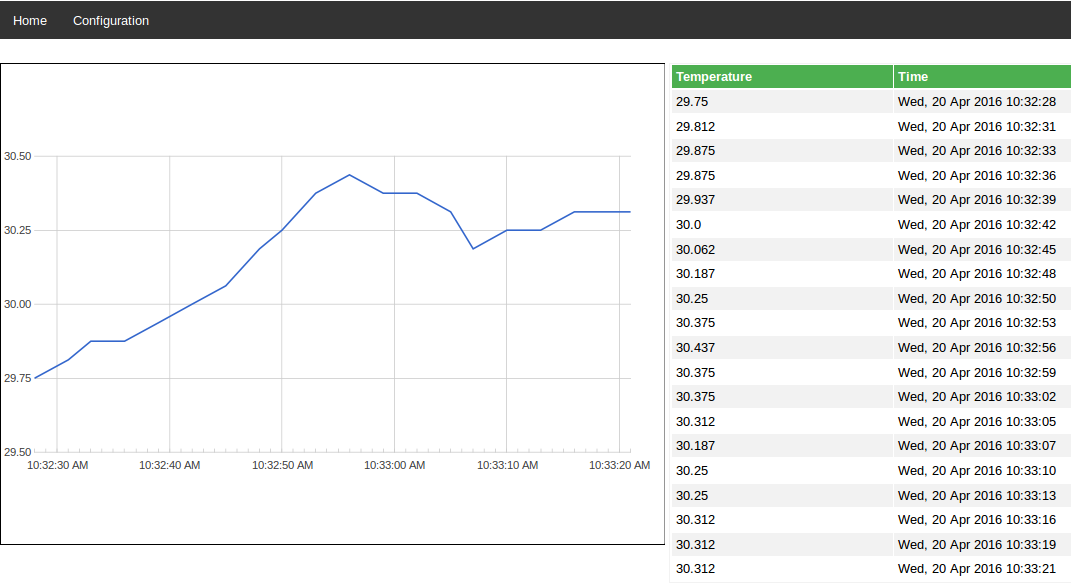
\includegraphics[width=12cm]{fig/homepage.png}
		\centering
		\caption{Home page in the web application.\label{fig:homepage}}
		\end{figure}
		
		\subsubsection{Login}
		The login page allows the user to get access to the configuration page.

		\begin{figure}[h!]
		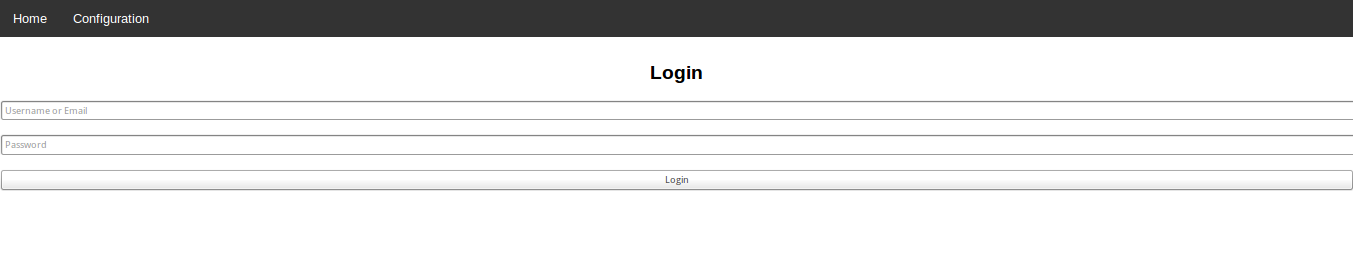
\includegraphics[width=12cm]{fig/loginpage.png}
		\centering
		\caption{Login page in the web application.\label{fig:loginpage}}
		\end{figure}

		\subsubsection{Configuration} %TODO poner que los modos se explican mas adelnate y enlazar, mirar si esta la config del ajuste de temperatura.
		The configuration page allows to change the device behaviour. The configurations that user can change are the scp target address, the frequency of the samples, the number of samples the web page show, the size of the data files stored in the device and the power saving mode. In this last configuration the user can change between 4 power saving modes, in the mode 2 and mode 3 the user also have 3 ways of input the schedule of the power saving modes, one where the interval of time is the same for all days, other where the user can input a different interval for every day of the week and also a last one where the user can input multiple intervals for each day.

		\begin{figure}[h!]
		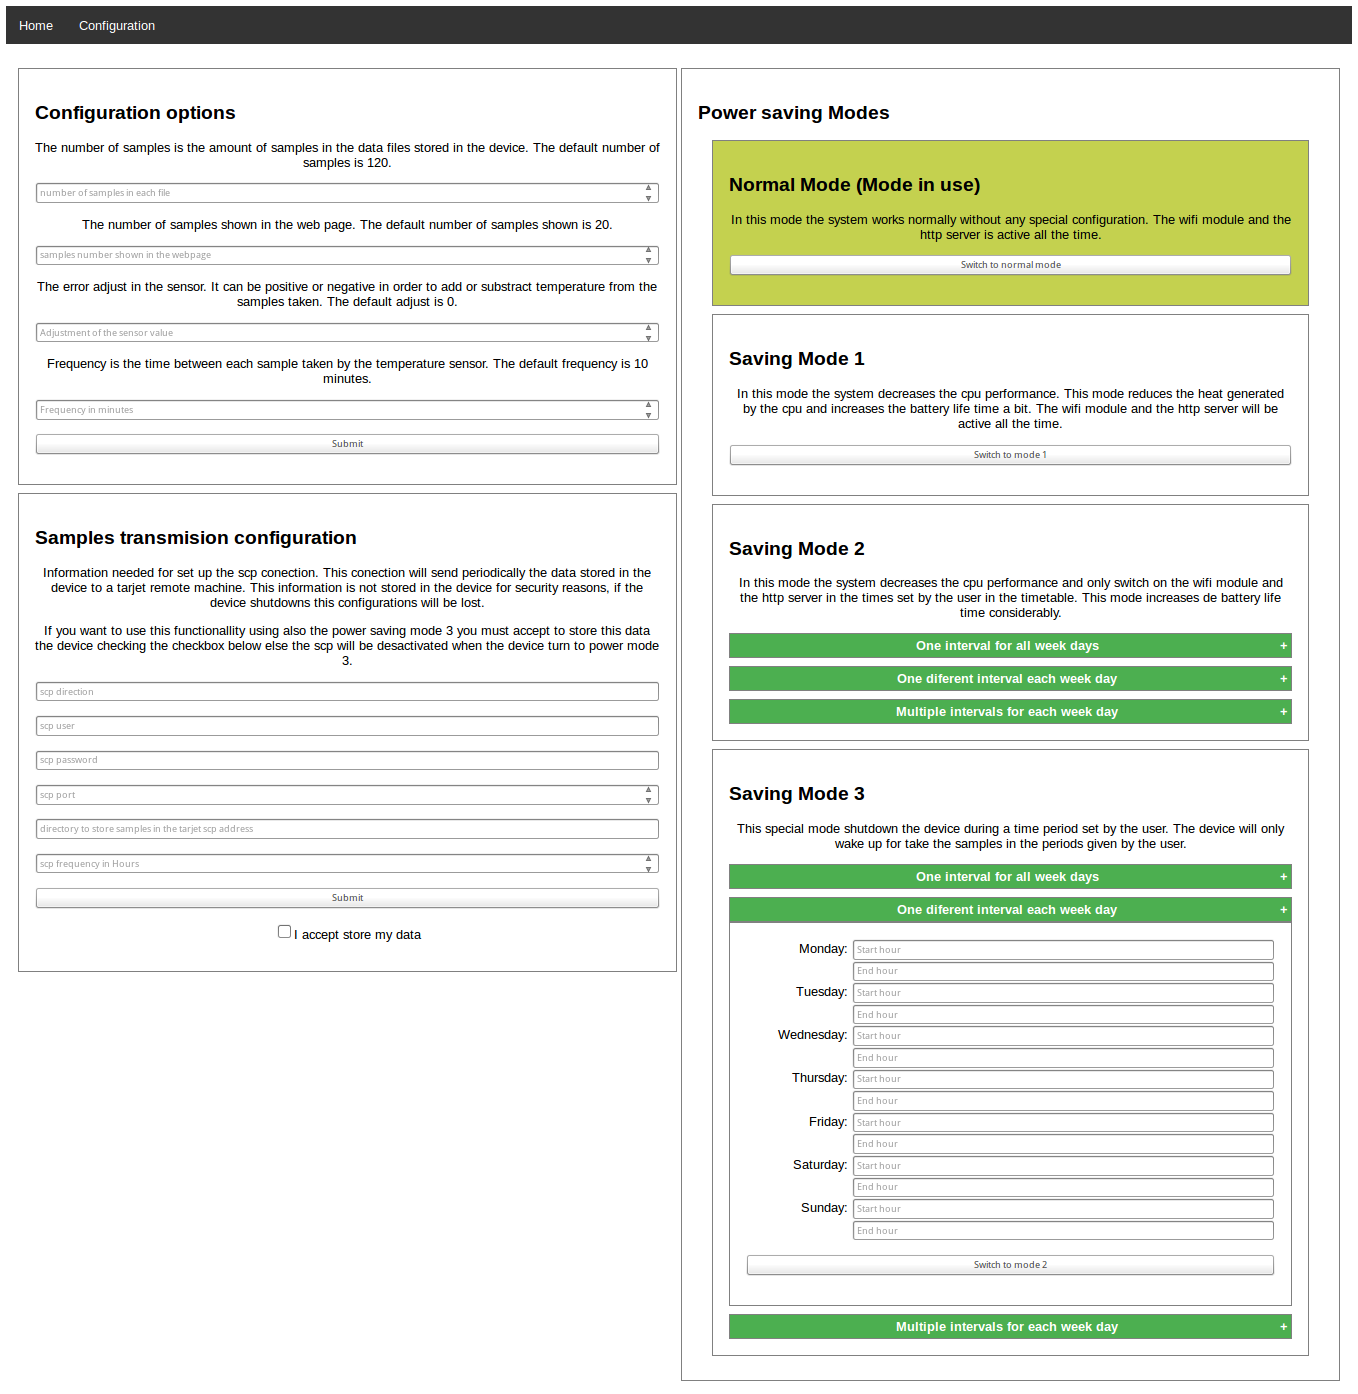
\includegraphics[width=12cm]{fig/configurationpage.png}
		\centering
		\caption{Configuration page in the web application.\label{fig:configurationpage}}
		\end{figure}

		The configuration page shows always what power saving mode is actually set up in the device configuration. Because the web server only serve static content there is 4 html files for the configuration stored in the device. Each one of these files change the actual selected mode. This is not a clever solution for big and complex web pages but in our case there is only four options which only change the class of one element whitouth any other collateral consequence and thanks to this solution we can save battery of the device avoiding add programs which precompile the html files or another complex solutions.

		\subsubsection{Error Page}
		Another important matter was give feedback about errors to user when the data input was not correct or when a internal problem happens. This is a main topic in a user interface and a static web server is so limited for give feedback to user.

		\begin{figure}[h!]
		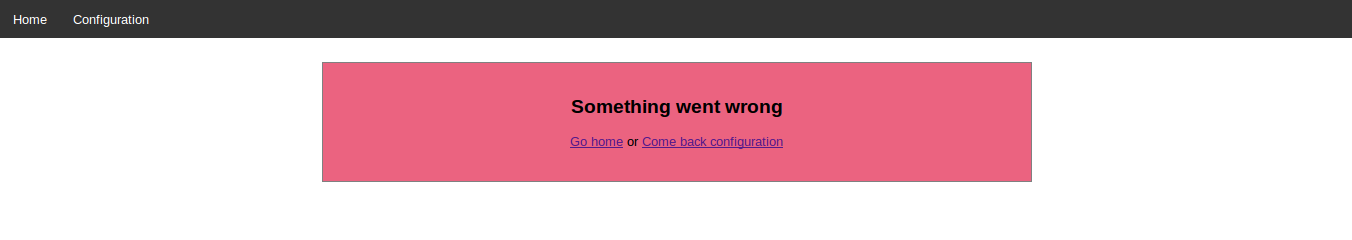
\includegraphics[width=12cm]{fig/errorpage.png}
		\centering
		\caption{Error page in the web application.\label{fig:errorpage}}
		\end{figure}

		For this problem is not possible to use the solution implemented in the configuration section for show the current power saving mode because the number of possible states is too big and during implementation the number of errors handled will grow for sure.

		For this problem the web application redirect the user to a generic web page with a text explaining the problem.

		\subsection{Scripts}
		With the aim of save battery sending so many data the web application was designed having in mind make a simple web page trying to use all the power of html5 functions and decreasing the number of scripts needed.

		For these reason there is only two scripts used in the web application.

		\subsubsection{configuration.js}
		The configuration script is only used in the configuration section. This script has two main functions. In one hand the script create a pop up asking confirmation to the user if the values introduced are between the allowed ranges but not so desirable in order to save battery or if the values are in conflict with another configurations. In the other hand the script create the accordions with the three ways for input the power saving mode 2 and 3 schedules.

		\subsubsection{chart.js}
		This script get the values of the samples directly from the html table of the html file and using that data the script generate the graphic in the home page.

		Also the script control the size of the window resizing the graphic for keep the responsive dessign.

		\subsection{Styles} %FIXME
		Although the web application is concerned in the functionality the dessign was made keeping in mind the user experience. Because there is strict requirement of energetic efficiency the dessign was made also avoiding send more data than necessary in every server request answer. For that reason there is no big dessign libraries stored in the device and the design strictly respect the KISS principle.

		The style is provided only for a simple css style sheet for all the web application which control the position of the elements and provide some media queries which implement a responsive design.

		\subsubsection{Responsive}
		Nowadays the way to use Internet is so different from four or five years ago. The smart phones changed completely the way to use web pages and now is mandatory to dessign not only a desktop web page but also a mobile dessign prepared for small screens. 

		%\begin{figure}[h!]
		%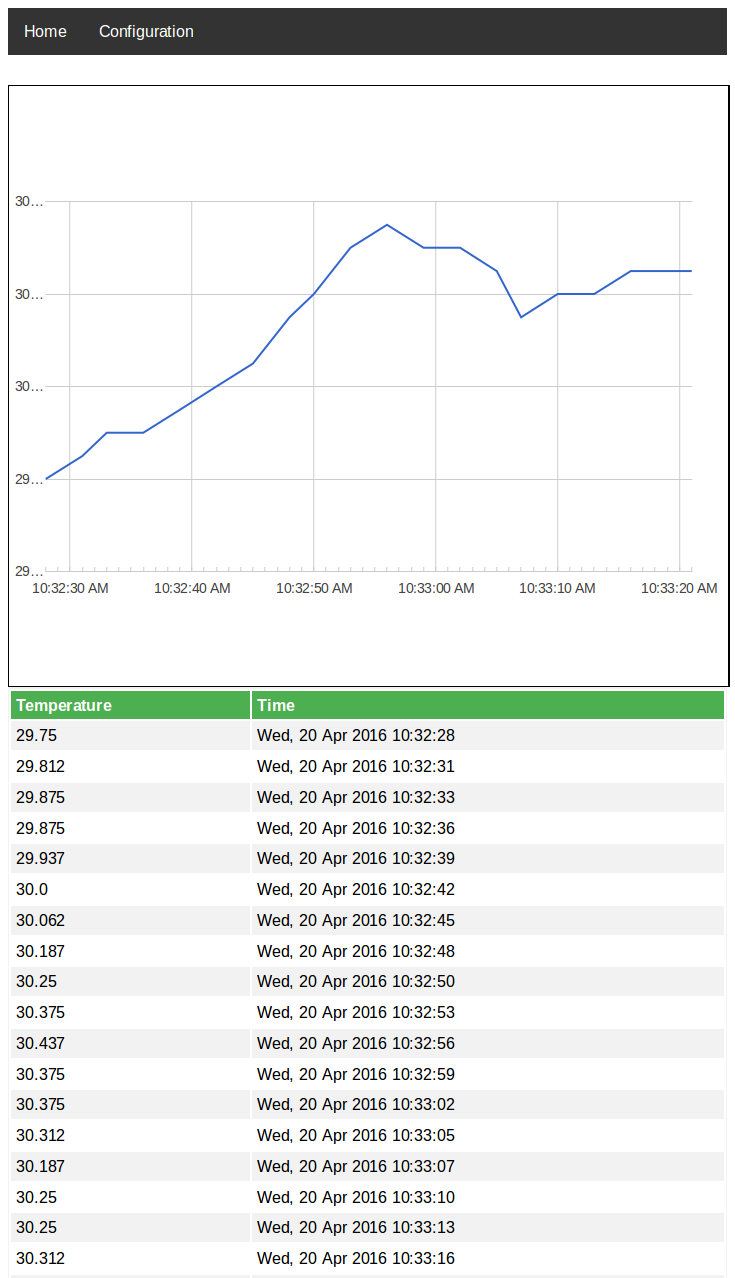
\includegraphics[width=8cm]{fig/responsive.png}
		%\centering
		%\caption{Responsive home page in the web application.\label{fig:responsive}}
		%\end{figure}

		For this objective there are media queries implemented in the style sheet which permit adapt the content to smaller screens changing what is show and where maintaining a understandable and clean dessign.

		\subsubsection{The style sheet}
		The stylesheet is stored in the css folder in the project folder. In the style sheet there is coded a generic dessign for all the web application and specific dessigns for each web page.

		\subsection{Libraries}
		The web application has two dependencies with external libraries. One of the libraries JQuery and the other one is Google charts tool.

		The web page uses this two libraries because are stored in remote servers. That is a great advantage because we don't need to store it and also and the most important reason because the device doesn't need to waste energy sending the library files on each client request to the server which is a way to save battery and also computational power.

	\section{Power saving modes}\label{sec:powersavingmodes}
	The system implements four power saving modes which change the configuration of the device enabling or disabling some configuration, hardware and programs lowering the device functionalities but decreasing the power consumption in order to increase the battery life time of the device.
		\subsection{Why?}
		The project is designed for stay working using a battery as power supply during the most time possible. The big problem of this kind of system is the battery life time because are thought for be working during long periods. Normally this kind of devices works in devices with few computational power but with big battery life time like Arduino or another chips similar to Arduino. But with the arrival of the Internet of the things (IoT) is coming the necessity and also the possibility of more powerful devices like Raspberry Pi. 

		Is truth that Raspberry Pi is a device which consume so few power, and a big part of the Raspberry Pi community think that try to decrease the power consumption is a non sense. Contrary to this point of view this thesis try to optimize the power consumption of the device as much as possible in order to increase the battery life time of the device trying in the same process to test the raspberry pi as an embedded system.

		This is not an easy task because even if Raspberry Pi has a lower consumption for a computer continue consuming so much if we compare this device with other like the before mentioned Arduino.

		Make Raspberry Pi consume the same or less than systems like Arduino is of course impossible and it's not the aim of this thesis try to achieve that. The two type of systems are so different and the objective of both systems is not the same. Raspberry pi is for sure more powerful and is a multipurpose device which can work as a multimedia station or like an embedded system like this but the chips like Arduino are designed for be only embedded systems and for sure are better option thinking only in power consumption. The problem of this chips is the lack of computational power which does not permit them to create a web server or work above a complex operating system like Raspbian. This fact is not trivial since a complete operating system grants lots of services, security systems and also make the develop of applications significatively faster.

		With this facts in mind the next power saving modes were developed.
		\subsection{Description}
		All the power modes were implemented using bash scripts which can be use from any directory of the device if they are placed in the ~/bin folder of the device user.

		This scripts also call another python scripts if it is necessary and principally enable or disable the power of the hardware components which are not needed in the device.

		The power mode scripts not only disable the ethernet interface saving computational resources, also disable the bus which gives power to the component even when the interface is down saving in this way the power destinated to that interface.

		There are hardware components which are disabled always because they are not useful for this system like the HDMI port or the ethernet port. But for security reason there is a power saving mode which enable all the disabled components if necessary.

		\subsection{When}
		Every power mode is designed to be work in some specific part of the lifecycle of the device. The default power saving mode which will be active if there is not a configuration about that is the first power saving mode. 

		The zero power saving mode is only thought for special moments where the hdmi port or the ethernet wire could be necessary but is not thought for the normal lifecycle of the device.

		The other two power saving modes are designed as hard saving power modes which decreasing the device functionality significantly but increasing in the same way the battery life time. These modes will disable the Internet connection disabling also the web server in order to save the most battery possible. These modes are designed to work following a schedule set up by the user which as a rule can not be full time in order to let the user change to other modes and recover the control of the device at least a couple of hours every day.

		\subsection{PM0}\label{sec:pm0}
		The zero power mode is thought as a special mode which will enable another time all the hardware functionalities. This mode will increase the battery consumption to the maximum and for these reason is not designed to be working in the device.

		This mode is thought for maintenance of the device when it is necessary to connect the device to a screen and the HDMI port is needed to be enable.

		It is not recommendable to use this mode in the normal lifecycle of the device.
		\subsection{PM1}\label{sec:pm1}
		The first power consumption mode is the default power saving mode in the device, it will be set if there is not another configuration and this mode will be automatically enable when the device goes out of the second or third power saving mode.

		This power saving mode decrease the frequency of the CPU in order to decrease the power consumption. The truth is that the power consumption only decrease a bit but the collateral fact is that the heat generated for the CPU decrease also.

		Even if the power consumption decrease only a few with the lower CPU frequency is better than nothing and the heat decrease is useful in order to increase the life of the device and in order to avoid affect the temperature sensor samples.

		Of course this power saving mode also disable the HDMI and the ethernet port. It also would be so useful disable the USB hub letting active only the USB port used by the Wifi module but the way is dessign the hardware does not allow to make this because the USB ports are not independent ones of others, they are all connected to the same master usb root port like is explain in the \ref{subsec:powersave} section.

		\subsection{PM2}\label{sec:pm2}
		This power saving mode was designed thinking in extend the battery life lowering the device functionalities even if the connection with the device is lost in order of make possible get a device which can be working for longer periods.

		The main fact in this power saving mode is that the Wi-Fi module is disabled and the user won't be capable of connect with the device for change the configurations. If this power saving mode would be working without stop it wouldn't be useful because the user would need in some moment to be physically in front of the device, connect it to a screen and change the power mode manually.

		In order to avoid the necessity of g find the device for change the configuration this mode is not allow by the system to be working 24 hours every day. The user must set up a schedule for this power saving mode in the configuration page of the web application which using a crontab will manage the power saving mode automatically. The schedule will restrict the maximum time which the device can be in the second power saving mode, 23 hours is the maximum time for a day, permitting user to change the configuration at least one hour every day.

		This power saving mode will disable the same things disabled in the first power saving mode and also will disable the USB hub, the Wifi interface and the web server.

		As an exception, if the scp subsystem is running, it will detect if the second power saving mode is enabled, in this case the subsystem will enable the Wi-Fi interface in order to send the data to the target machine address and then it will disable the Wi-Fi interface another time.

		\subsection{PM3}\label{sec:pm3}
		In a harware system like raspberry pi is not possible to let running only the temperature subsystem in order to extend the battery life time if we don't use a special operating system which wouldn't allow us to run a web server and would be difficult and hard to develop or if we don't use special hardware like an Arduino connected to the Raspberry pi for example.

		With the objective to increse the battery life time extreamly the third power saving mode will shut down the device setting an alarm in an RTC module which will wake up the device just before take a temperature sample.

		When the device wake up first take the sample and then check if in the schedule set up by the user is time to change to another power saving mode or if the system have to shut down itself another time until next sample time. If it have to shut down another time, before this, the system set up a new alarm in the RTC which only can store one alarm at the same time.

		Like the second power saving mode, the third power saving mode follows a schedule set up by the user with the same rules and reasons as the second power saving mode.

		In this power saving mode the SCP subsystem will work only if the user mark the checkbox of the configuration web application accepting store the scp configuration data in the device, else the data will be lost on every shut down the device will do. Also if the scp configuration is stored in the device the scp data transfer frequency will not be followed and the subsystem will send the new data every time the device will wake up in order to do not lose data.

		\subsection{Another not implemented actions for decrease power consumption}
		%TODO hablar de cambiar componentes hardware, usar hardware especial para mejorar el rendimiento de la placa o permitir hibernar el dispositivo como dios manda.
	\section{Boot} %TODO improve
	As one important part of the system there is a boot script which on every boot of the device will check the configurations and will configure the device in order to keep the device working on the proper way.

	This script is written in bash and is called from /etc/profile configuration file on every boot. when the script is called it will change the actual location to the system folder and then it will execute the weaterStation.py python script. This last script is the one which will set up the actual configurations in the subsystems and also change the hostname of the device and the links of the html files in order to keep the device accessible from outside the university network.

\chapter{Life cycle} %TODO enalzar aqui las cosas a sus secciones.
	The system is designed to working continuously, without stop. During the working time the system will determine the state according to the power saving modes and the user new configurations.

	Also the system is conformed by three semi-independent subsystems which will perform different task, every subsystem has its own lifecycle which will be conditioned by the general system lifecycle and the user inputs.

	\section{Life cycle attending to Power modes}
		The lifecycle of the system is determine by the actual power mode, the change between power modes changes the behaviour and the functionalities of the system. Also the change between power modes will determine directly the movement between states in the subsystems.

		Initially the system will boot, in this moment the system will execute the boot script which will make the system jump to the actual state checking up the actual power mode for set up the right configurations in the system according to the actual power mode.

		The number of possible initial states where the system can jump after the boot checks are four and represent the four different power saving modes.

		\subsection{Change between states}
		The are two possible ways to change between states. One is manually, the user will input some configuration data which will determine the new state of the system. The other one is automatically, the user will input some configuration data which will determine the behaviour of the system during certain intervals of time.

			\subsubsection{Manual changes}
			In this system the user is capable of change the device state manually during certain intervals of time.

			For this aim the user can use the web application in order to change the configuration of the device. The web configuration page has to types of possible configurations. In one side there are the system state configurations which will change the system state. In the other side there are the subsystem configurations which will affect the subsystems behaviour but not their state.

			The configurations that will affect the system state are the power saving mode configurations. Setting up the different power saving modes the system will jump between states affecting the behaviour and functionalities of the system.

			Depending on the state it is possible that this state change way will not be accessible. In the second power saving mode it is possibly disabled if the network interface is disabled and also in the third power saving mode when the device is sleeping.

			\subsubsection{Schedulled changes}
			The scheduled or automaticall state change happens in the second and third power saving mode when the user had set up a schedule which will determine the state of the system depending on the actual date of the device.

			For this reason the device will write a crontab which will automatically change the state of the device following the user input.

			The change between states is limited in this mode and also depends if the enabled power saving mode is the second one or the third one.

			In the scheduled changes of the second power saving mode the possible jumps are from the second power saving mode state to the first power saving mode state and from the first state to the second.
			
			\begin{figure}[h!]
			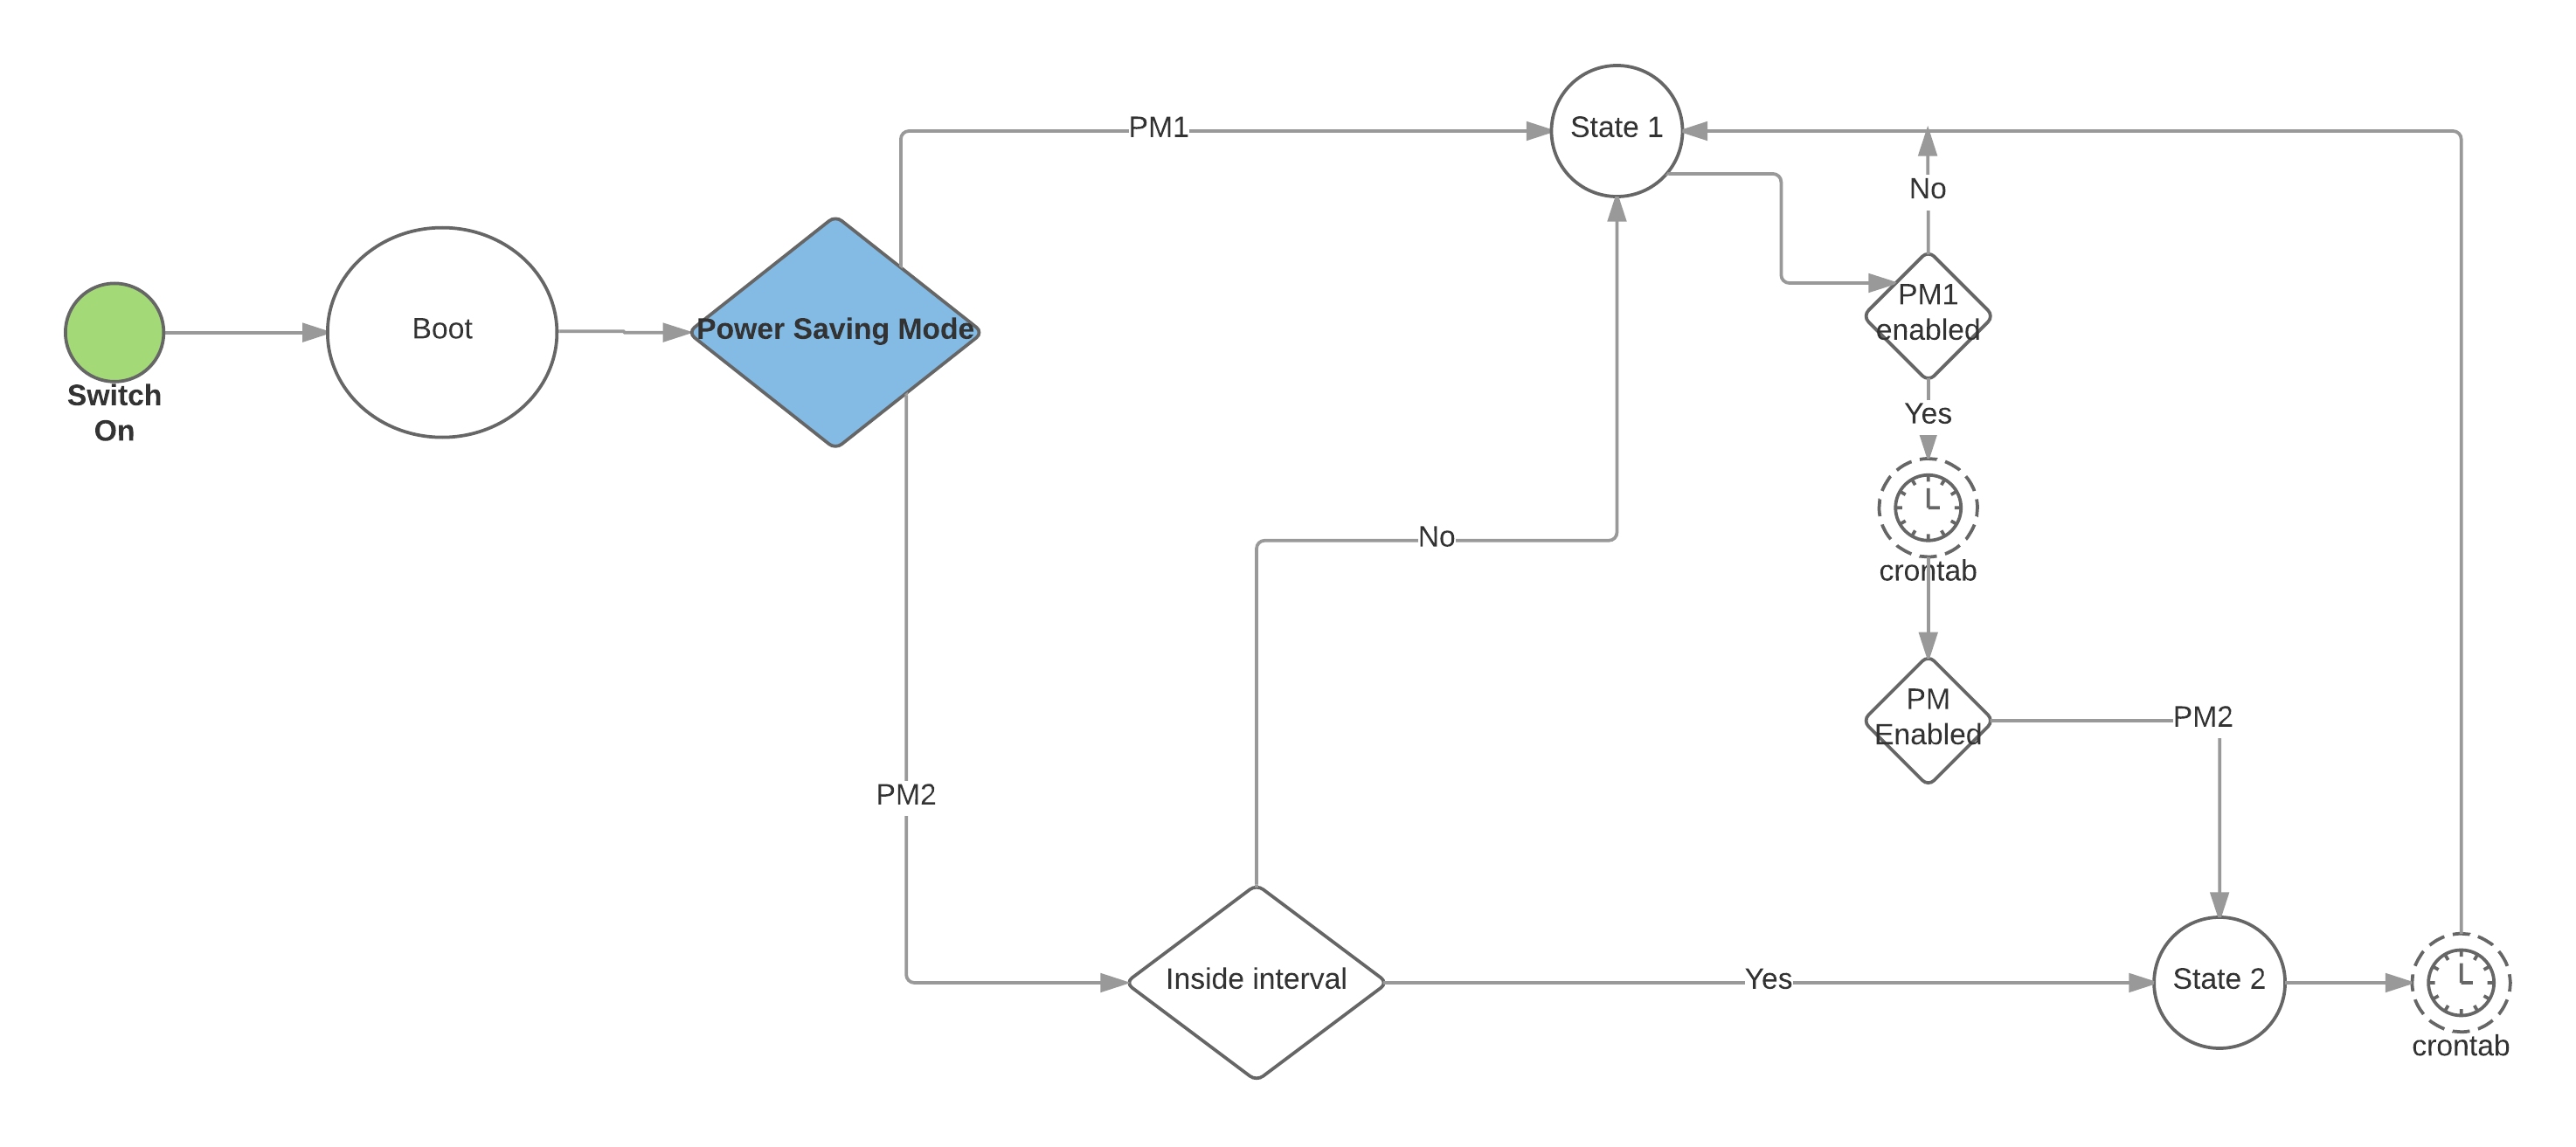
\includegraphics[width=8cm]{fig/states-pm2.png}
			\centering
			\caption{Second power mode state diagram. \label{fig:pm2}}
			
			\end{figure}

			Also in the scheduled changes of the third power saving mode the possible jumps between states are from the the third state to the sleep state and from the third state to the first state.
			
			\begin{figure}[h!]
			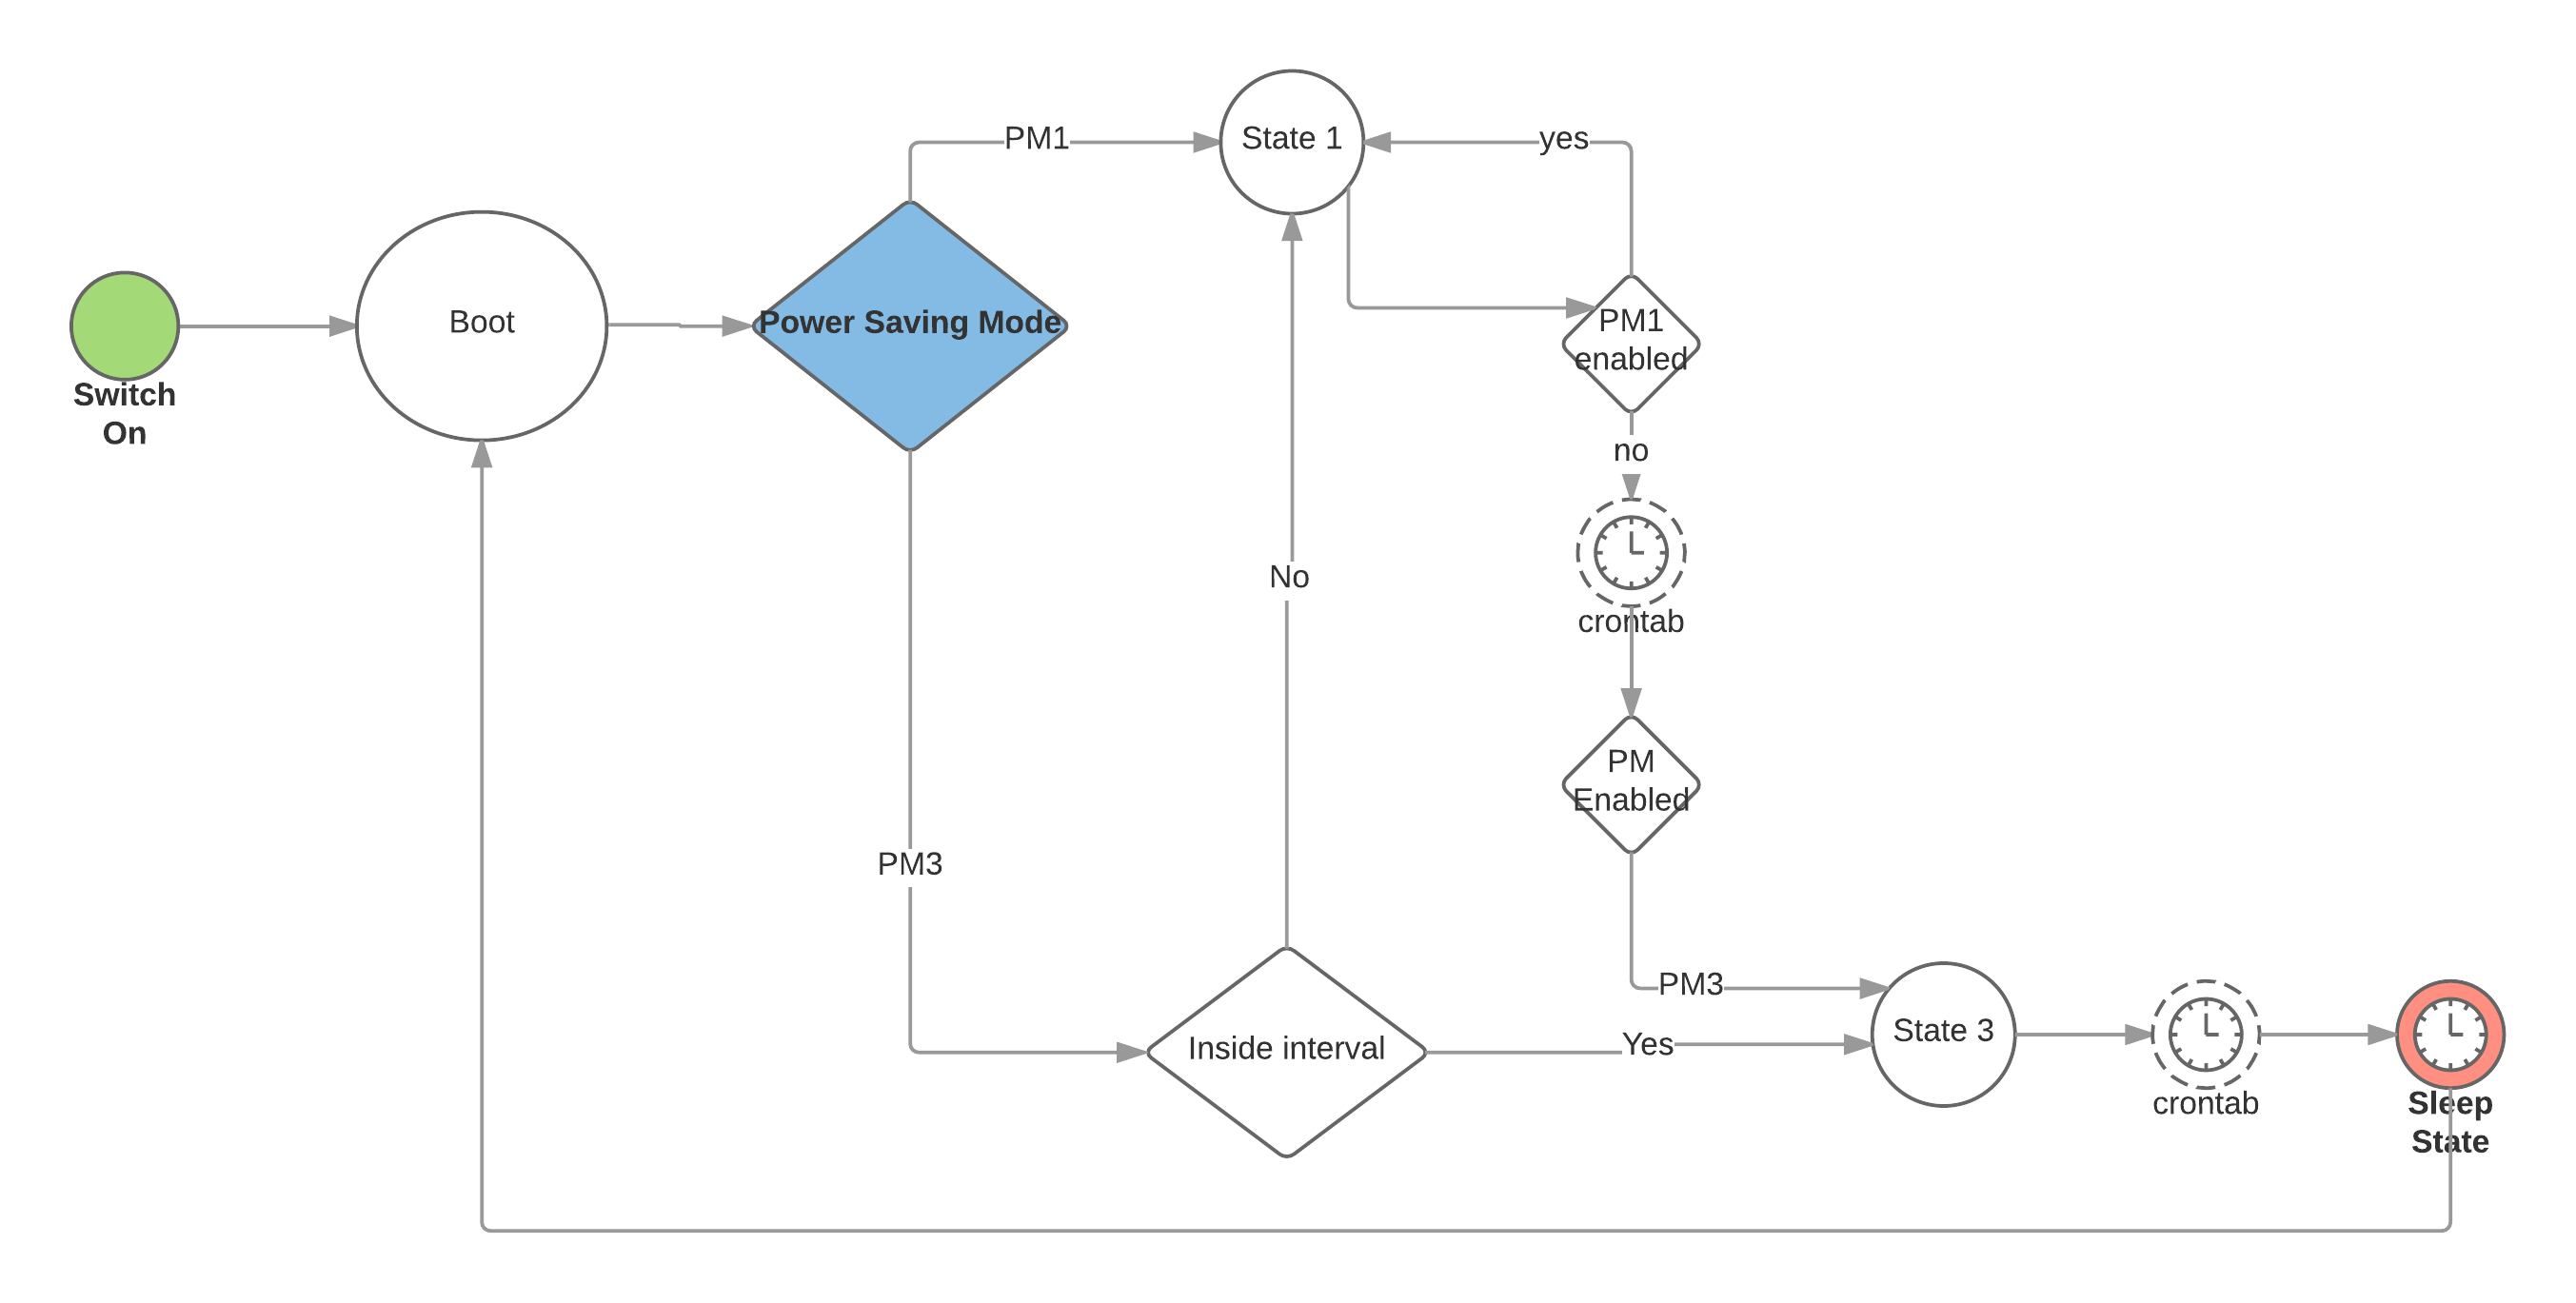
\includegraphics[width=8cm]{fig/states-pm3.png}
			\centering
			\caption{Third power mode state diagram. \label{fig:pm3}}
			\end{figure}
			
		\subsection{States Diagram}

		How it is possible to watch in the figure \ref{states} once the device is switch on it enter in a boot state where the system check the configuration files. In function of the actual power saving mode state the system can jump to 4 different states. The state 0 corresponds to the normal power saving mode which represents the device without any special configuration in order to save battery life was explained in section \ref{sec:pm0}. In the same way the state 1 corresponds to first power saving mode, state 2 to second power saving mode and state 3 to third power saving mode.

		From the state 0 it is not possible to change to another state without the interaction of user in the web application.

		From the state 1 it is possible to jump to state 2 if the second power mode is enabled or state 3 if third power saving modes is enabled, both jumps happen when and a scheduled cron job occurs. If the enabled power saving mode is the first one it is not possible to jump to another states.

		\begin{figure}[h!]
		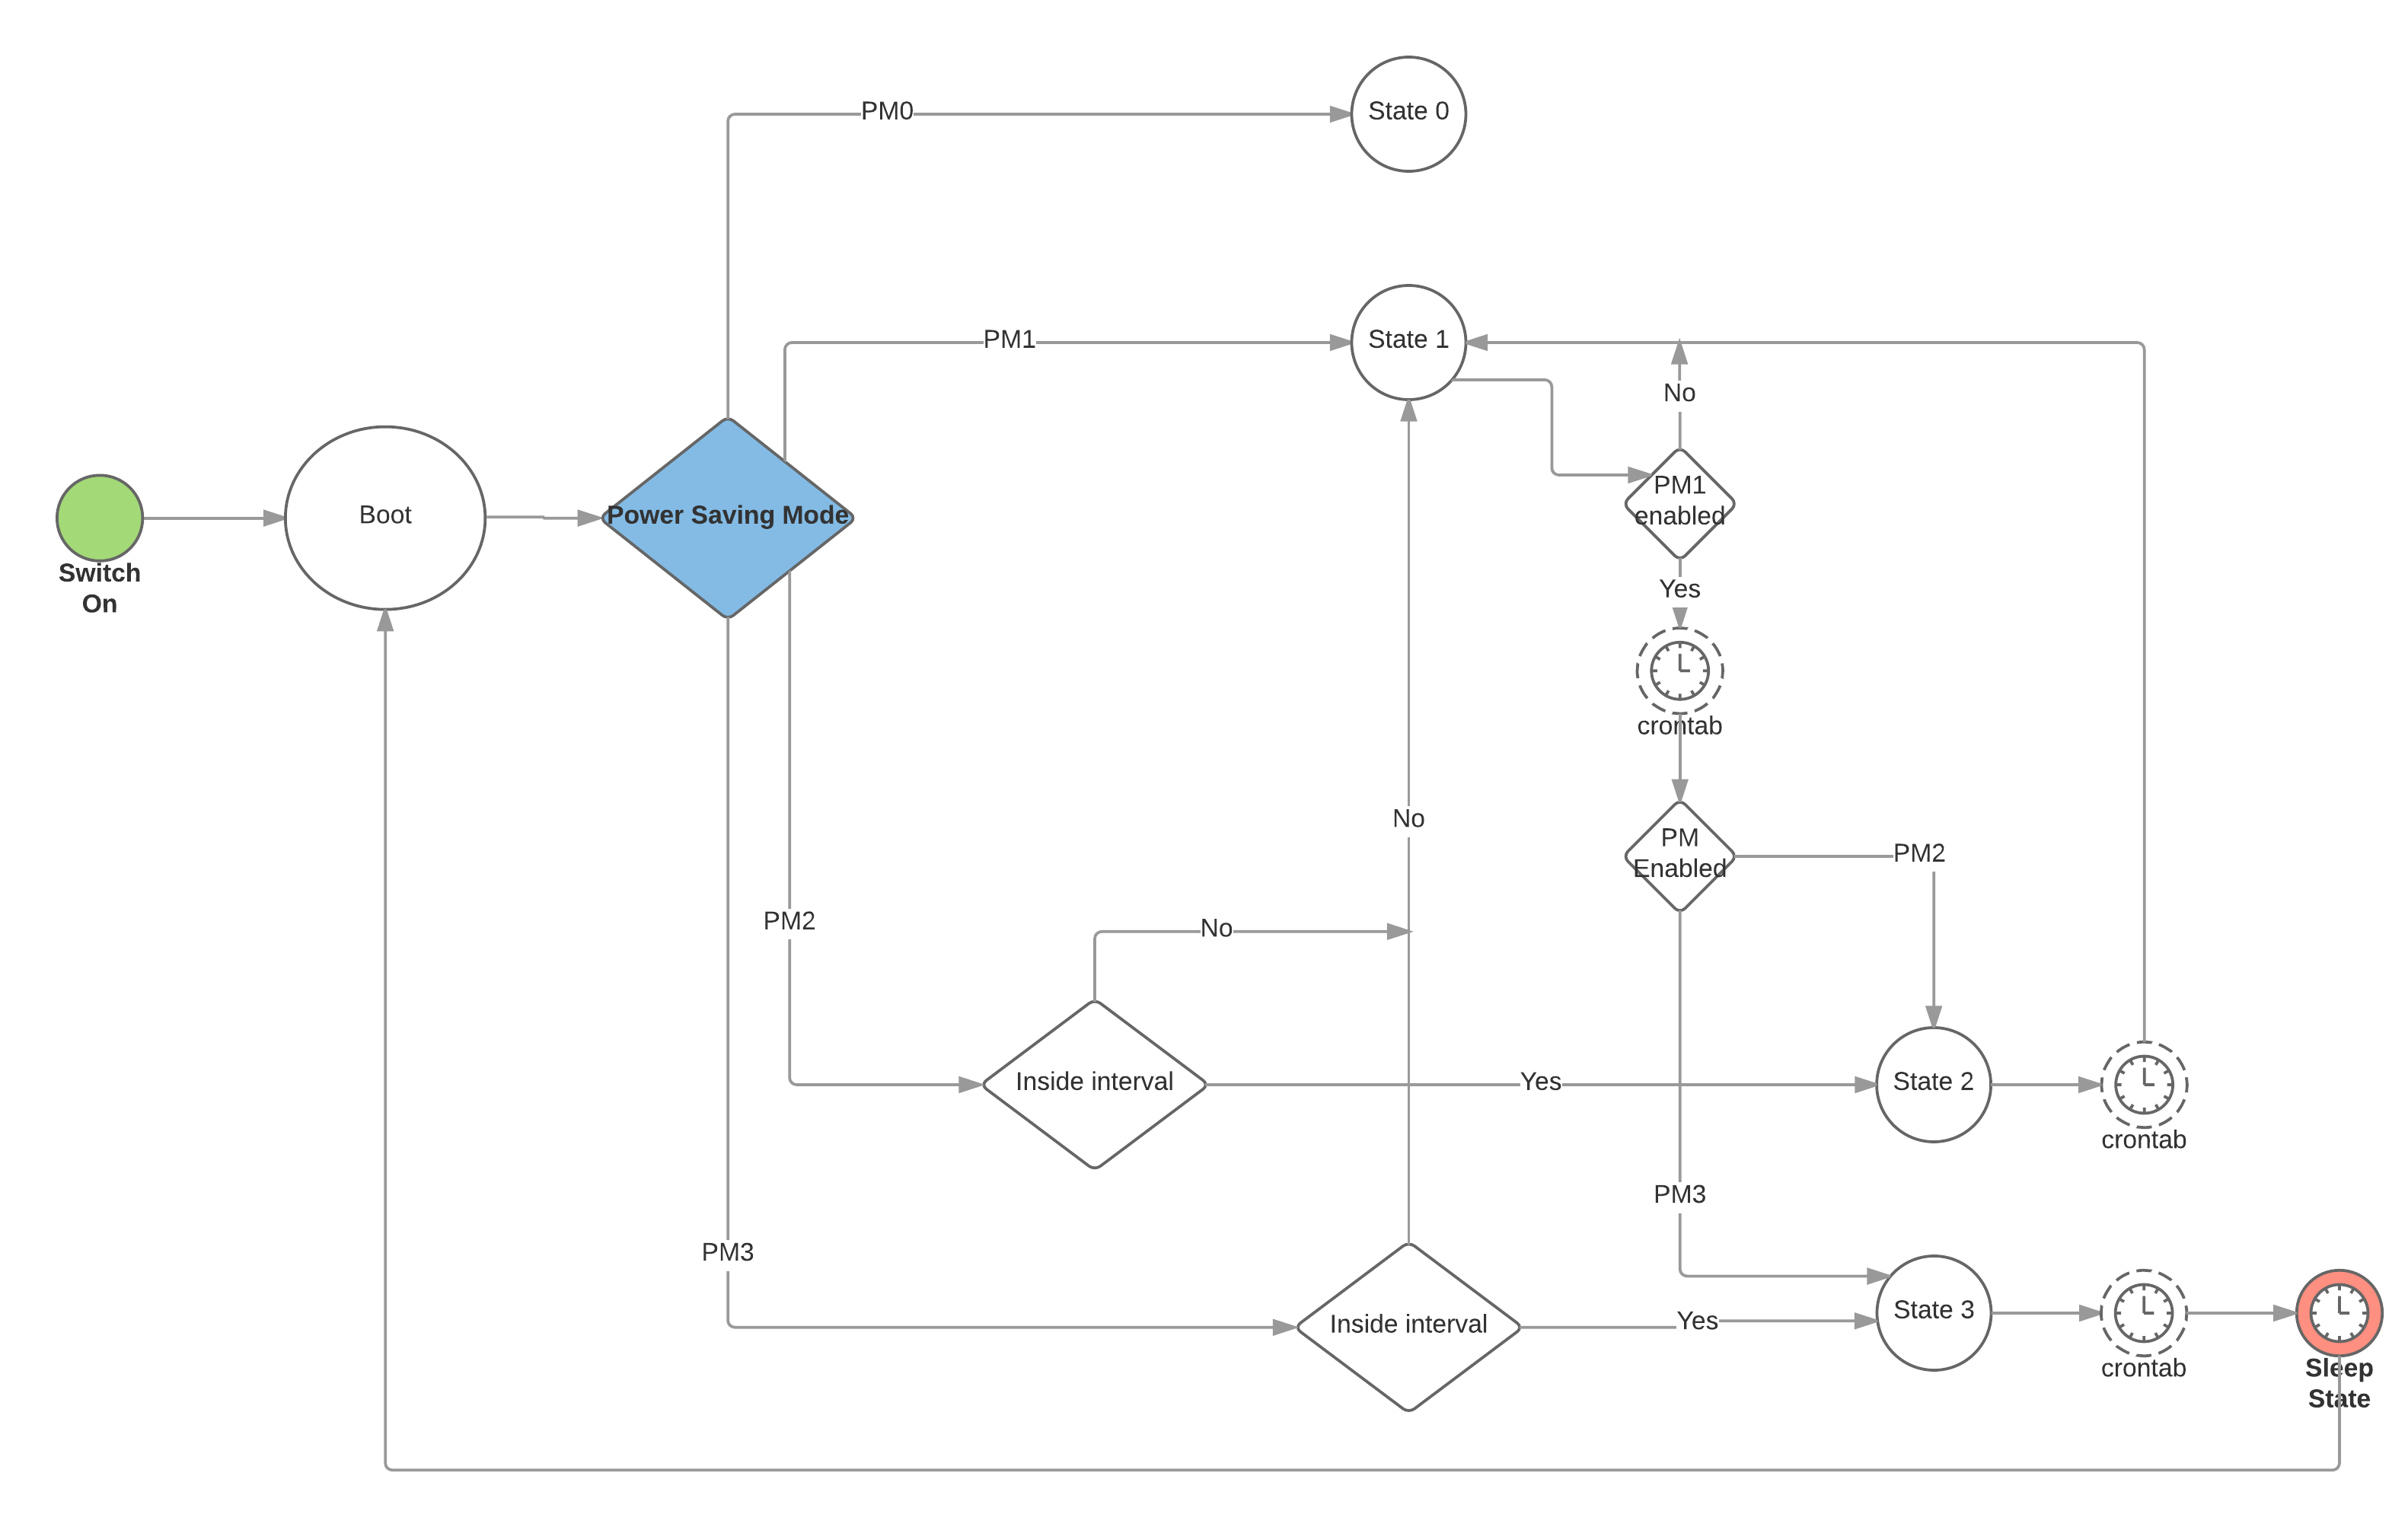
\includegraphics[width=8cm]{fig/states-pm-complete.png}
		\centering
		\caption{Complete state diagram.\label{states}}
		\end{figure}

		From the state 2 is possible to jump to the state 1 when the scheduled cron job happens.

		And from state 3 when the scheduled cron job occurs the system will jump to a sleep state. In this state the device is shut down waiting for the RTC clock module alarm to wake up. When the RTC alarm occur the device wakes up and enter in the boot state where the state will redirect the system to the state 0 or to the state 3 depending of the device time and the scheduled cron jobs for the device.
		%TODO aqui se puede poner que pm3 es muy cortito igual que boot

	\section{Life cycle attending to subsystems}
	The system is composed by three main subsystems as is written in the chapter \ref{chap:software}. These principal subsystems are the temperature subsystem which measure the temperature every certain time set up by the user, the scp subsystem which transfer the raw data to a target machine and the web server subsystem which show the data and allow the user to change the device configuration. Every subsystem has its own lifecycle directly influenced by the general system lifecycle and the user configurations.

	\subsection{Temperature and SCP subsystems lifecycle}
	This two subsystems share the basic structure of their code is that for the reason i prefer to explain their lifecycles as the same because the states where they can stay are the same. The only difference between their lifecycles is the event which starts the lifecycle.

	\begin{figure}[h!]
	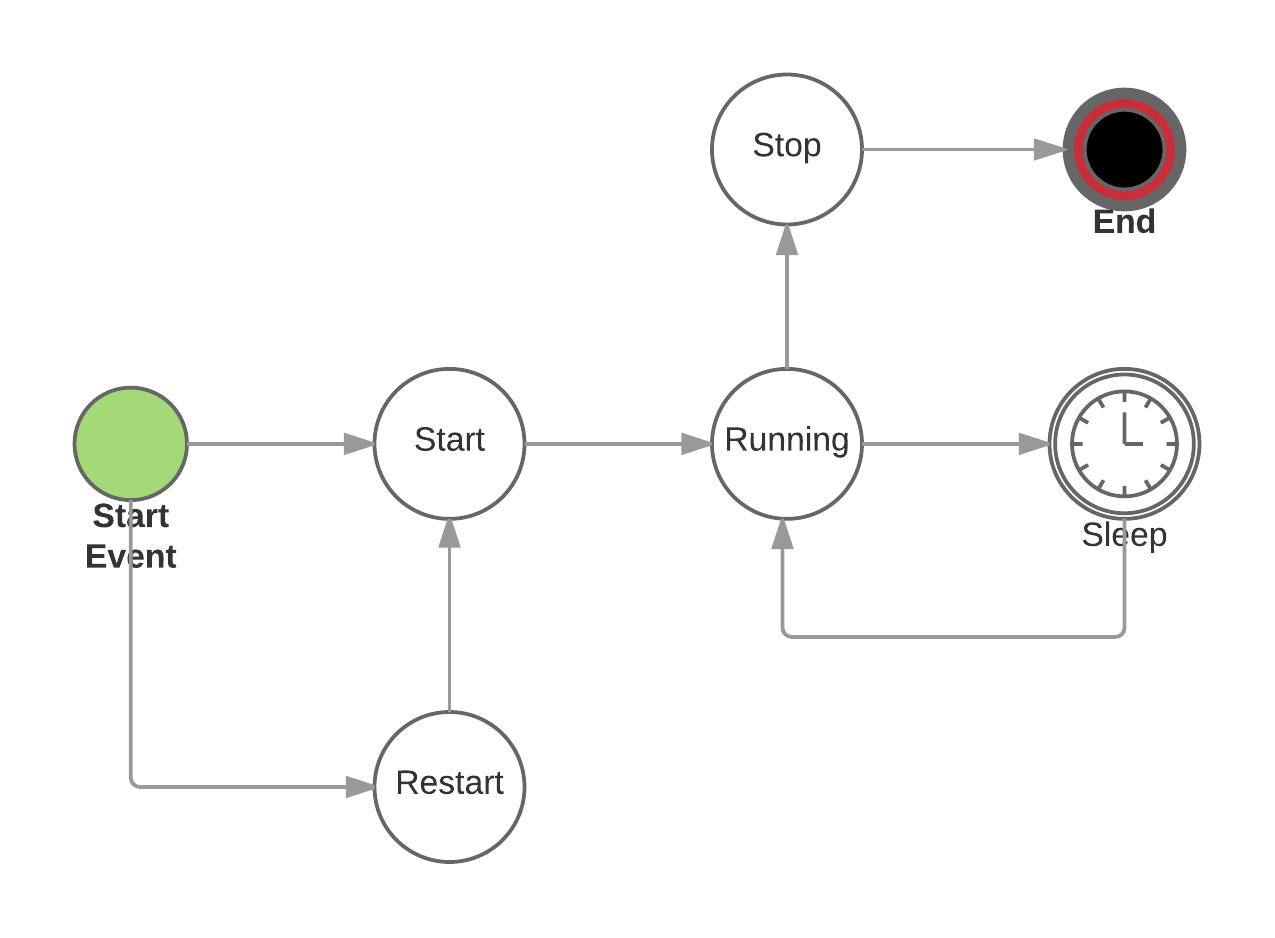
\includegraphics[width=8cm]{fig/daemon.png}
	\centering
	\caption{SCP and Temperature subsystems state diagram.\label{states}}
	\end{figure}

	Firstly, the start event in this two subsystems is a call from the boot state of the system. The boot state check the configurations and depending of these configuration value it will wake up the subsystems or not. In the temperature sensor case the start event will always come from the boot state of the system. The boot state will wake up the temperature subsystem always. In the other hand the boot state will wake up the scp system only if exist a configuration file which contains the necessary data for it. If this configuration file does not exist the only other event which can start the scp lifecycle is the set up of the scp data in the configuration section of the web application.
	\\
	\\
	After this start event the lifecycle diagram is completely the same for both. Once the initial event wakes up the subsystem it jumps to the start state, in this state the subsystem checks some configurations and make some initial task in order to initialize itself. Then the subsystem jumps to the running state where it performs it task and jumps to a sleep state during a certain time set up by the user in the configurations. When the subsystem wake up from sleep it make another time the same task and return to the sleep state in a infinite loop. This loop only will be break when the system kill the subsystem directly or in a indirect way when it shut down the device. %TODO fixme, no me gusta la ultima parte en la que no se menciona el estado de stop

	\subsection{Web server subsystem lifecycle} %TODO referencia boot state
	The web server subsystem has a quite easy lifecycle. As a server, when it starts running it will be working without stop until the system will kill it. 

	The subsystem will be wake up by the system only when the system jump to the state 0 or the state 1. That means that the web server will be wake up in all the power saving modes when they are in state 1, or in state 0.

	And also the subsystem process will be killed when the system jumps to state 2 or state 3 which means that there is no network interface enabled and for this reason is a no sense keep the process alive.

\chapter{Real world uses \& Conclusions}
	\section{Improvements}
	%hablar de lo de que se puede desactivar los datos en los puertos para que no se conecte la gente sin permiso
	%mejorar lo del auto wake up
	%puede ponerse que la raspi con su potencia de calculo podria genrar todo tipo de estaidsiticas complejas, predicciones, avisar de posibles picos de temperatura o simplemente generar datos en grueso
	%tratar con el scp, podria servir para que otra maquina procese los datos que esta genera
	\section{Real world uses}
	%generar datos que otras maquinas procesen y usen para cambiar su comportamiento
	%podria ser un termostato inteligente
	%señal de traffico que avise de heladas en la carretera o del calor
	\section{Conclusions}
	%hablar de la raspi como no muy efficiente en este ambito, en como podria haberse hecho, mandando datos a un servidor que los muestre etc.




